% ---------------------------------------------------------------------------- %
\subsection{Die Steuerung}
% ---------------------------------------------------------------------------- %

Unter einer Steuerung  versteht man eine offen Wirkungskette  wie in Abbildung
\ref{fig:Steuerung},   dass  heisst   die  Wirkglieder   sind  ketten\"ahnlich
aufgereiht und besitzen keine R\"uckkopplung. Die Steuerkette wird genau f\"ur
eine Steuerung ausgelegt und kann  nur auf Steuergr\"ossen reagieren. Ohne die
R\"uckkopplung wird das Ausgangsignal  nicht mit dem Eingangssignal verglichen
und es k\"onnen keine Korrekturen vorgenommen werden.

\begin{figure}[!h!, width=\pagewidth]
    \centering
    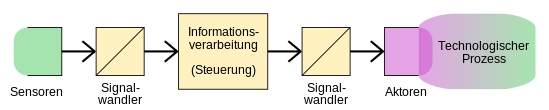
\includegraphics[width=0.5\textwidth]{images/Steuerung}
    \caption{Steuerung}
    \label{fig:Steuerung}
\end{figure}


% ---------------------------------------------------------------------------- %
\subsection{Der geschlossene Regelkreis}
\label{subs:grundl:geschlossenerRegelkreis}
% ---------------------------------------------------------------------------- %
Die      Aufgabe     eines      geschlossenen     Regelkreises      (Abbildung
\ref{fig:geschlossenerRegelkreis})  ist  es,   einen  vorgegeben  Sollwert  zu
erreichen und diesen  auch bei St\"orungen aufrecht  zu erhalten. Dabei sollen
die unten  genannten dynamischen  Anforderungen eingehalten werden,  damit die
Stabilit\"at des Regelsystems garantiert ist. Daraus folgt auch die wichtigste
Bedienung f\"ur  die Schrittantwort ein geschlossenen  Regelkreis heisst, dass
der Regelfehler, die Differenz zwischen Ist- und Sollwert, m\"oglichst schnell
gleich Null oder m\"oglichst klein ist.


\begin{figure}[!h!, width=\pagewidth]
    \centering
    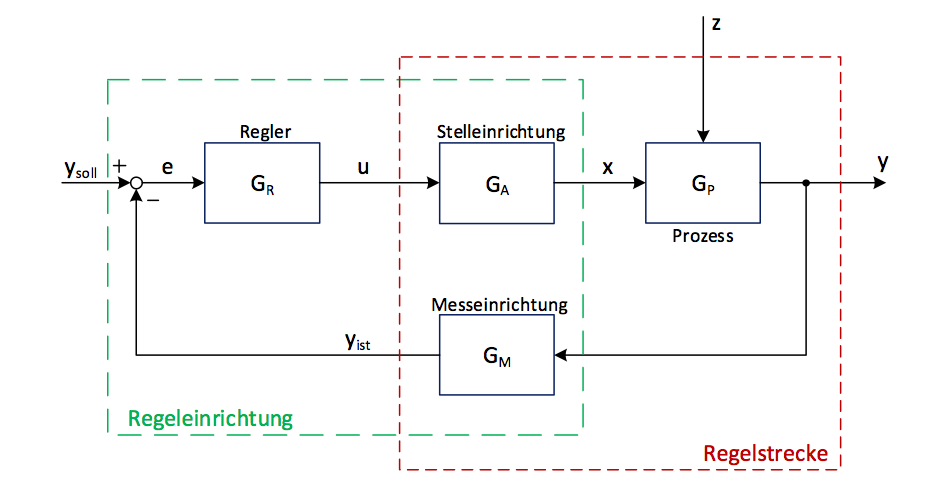
\includegraphics[width=0.5\textwidth]{images/geschlRegelkreis}
    \caption{Geschlossener Regelkreis}
    \label{fig:geschlossenerRegelkreis}
\end{figure}

%Name Bild Struktur eines allgemeinen Regelkreises
\begin{itemize}
    \item
        $y_soll$ bezeichnet den Sollwert der Regelgr\"osse
    \item
        $e$ Regelabweichung (Regelfehler)
    \item
        $u$ Steuergr\"osse
    \item
        $x$ Stellgr\"osse
    \item
        $y$ Regelgr\"osse
    \item
        $z$ St\"orgr\"ossen werden in diesem Projekt nicht ber\"ucksichtigt
    \item
        $y_ist$  ist der  Ist-Wert der  Regelgr\"osse  und wird  auch als  die
        Schrittantwort des Regelkreises bezeichnet.
\end{itemize}


Grunds\"atzlich  k\"onnen  f\"unf   Anforderungen  f\"ur  einen  geschlossenen
Regelkreis und seinen Schrittantworten zusammengefasst werden:
\begin{enumerate}
    \item
        Der Regelkreis muss stabil  sein: F\"ur das Regelsystem heisst stabil,
        dass es in seinen Gleichgewichtszustand zur\"uckgef\"uhrt werden kann.
    \item
        Der Regelkreis muss gen\"ugend ged\"ampft sein.
    \item
        Der   Regelkreis   muss   eine  bestimmte   station\"are   Genauigkeit
        aufweisen: Das   bedeutet,    der   Regelfehler   e(t)    soll   f\"ur
        $t\rightarrow\infty$ gegen null gehen.
    \item
        Der  Regelkreis  muss  hinreichend schnell  sein: Ist  die  D\"ampfung
        zu  stark   oder  zu  schwach,  braucht   der  Einschwingvorgang  mehr
        Zeit. Hierbei  muss  darauf  geachtet werden,  dass  die  spezifischen
        Anforderungen an das Regelsystem eingehalten werden.
    \item
        Der  Regelkreis muss  robust  sein: Der Regelkreis  muss so  ausgelegt
        werden,  dass  das  Regelsystem  auch im  schlimmsten  Fall  (je  nach
        Regelsystem situationsabh\"angig) in der Lage ist, das System zur\"uck
        in den stabilen Zustand (vgl. 1.) zu regeln.
\end{enumerate}


% ---------------------------------------------------------------------------- %
\subsubsection*{Die Schrittantwort des geschlossenen Regelkreises}
% ---------------------------------------------------------------------------- %

\begin{figure}[h!, width=\pagewidth]
    \begin{center}
    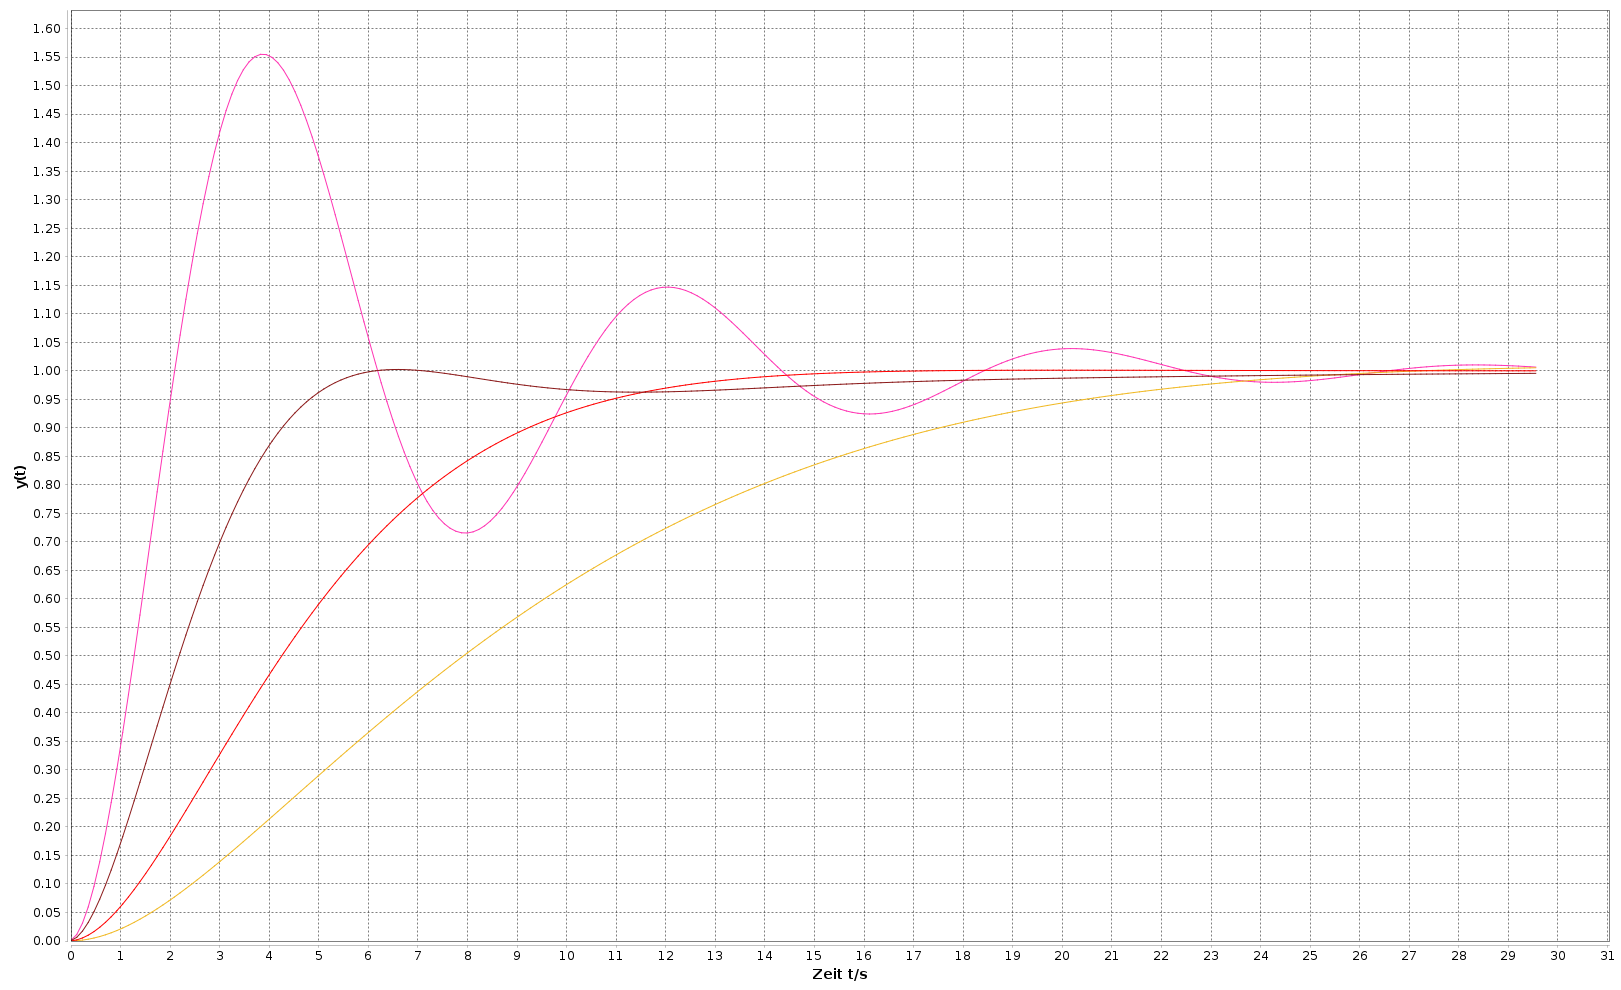
\includegraphics[width=0.8\textwidth]{images/schrittantworten.png}
    \caption{Schrittantworten verschiedener Charakteristiken}
    \label{fig:stepresponse}
    \end{center}
\end{figure}

Als Schrittantwort eines geschlossenen Regelkreises wird der zeitliche Verlauf
des Ausgangssignals  $y(t)$ bezeichnet,  welches entsteht wenn  $y_{soll}$ von
$0$  auf  $1$ springt. In  der  Abbildung  \ref{fig:stepresponse} werden  drei
verschiedene Schrittantworten gezeigt.  Im  Zusammenhang mit den Anforderungen
an  den  geschlossenen  Regelkreis,  werden  an  die  Schrittantwort  folgende
Forderungen gestellt:

\begin{enumerate}
    \item
        Die Schrittantwort eines stabilen Regelkreises darf nach dem Erreichen
        des eingeschwungenen Zustands kein erneutes \"Uberschwingen auftreten.
    \item
        Die  D\"ampfung  der  Schrittantwort  soll so  stark  sein,  dass  der
        eingeschwungene Zustand m\"oglichst rasch erreicht wird ohne, dass das
        \"Uberschwingen des Systems zu stark  wird. Die dunkel orange Kurve in
        Abbildung \ref{fig:stepresponse} zeigt eine Schrittantwort, welche vor
        dem Erreichen des eingeschwungenen Zustands, \"uberschwingt.
    \item
        Die   Schrittantwort  muss   f\"ur  ein   $t\rightarrow\infty$  gleich
        $y_{soll}$ sein.
    \item
        Die Schnelligkeit des Einschwingvorganges der Schrittantwort ist stark
        von der  D\"ampfung abh\"angig. Wenn  diese zu  stark oder  zu schwach
        ist, ist der Regelkreis zu langsam. Die hell orange Kurve in Abbildung
        \ref{fig:stepresponse} zeigt eine zu langsame Schrittantwort.
\end{enumerate}

Die  Berechnung   der  Schrittantwort  des  geschlossenen   Regelkreises  wird
in  unserem   Tool  mittels  der  inversen   schnellen  Fourier-Transformation
durchgef\"uhrt, genauere  Informationen dazu sind in  Anhang~\ref{app:fft} und
Anhang~\ref{app:algo:ifft} zu finden.


% ---------------------------------------------------------------------------- %
\subsection{Regelstrecke}
% ---------------------------------------------------------------------------- %

In  der  Regelungstechnik  wird  die  zu  regelnde  Strecke  als  Regelstrecke
bezeichnet. Die  zu   regelnde  Strecke   ist  zum  Beispiel   die  Temperatur
im  Raum  oder  die  Luftfeuchtigkeit  in  der  Sauna. Die  Regelstrecke  wird
durch  ihr   Zeitverhalten  charakterisiert,  welches  den   Aufwand  und  die
G\"ute   der   Regelung   bestimmt. Um  das   Zeitverhalten   zu   beschreiben
verwendet  man die  Sprungantwort,  welche zeigt,  wie  die Regelgr\"osse  auf
Stellgr\"ossen\"anderung reagiert. Mit  der entstehenden  Regelgr\"osse werden
verschiedene Regelstrecken unterschieden:

\begin{itemize}
    \item
        P-Regelstrecke
    \item
        I-Regelstrecke
    \item
        Strecken mit einer Totzeit
    \item
        Strecken mit Energiespeicher
\end{itemize}

Dieses  Projekt   besch\"aftigt  sich   mit  den  PTn-Strecken,   welche  eine
Kombination  aus einer  Strecke  mit proportionalen  Verhalten  und einer  mit
Totzeit ist. Die Ordnung der Strecke ist in n angegeben.

\subsubsection*{P-Regelstrecke}
Bei  der  Regelstrecke mit  proportionalem  Verhalten  folgt die  Regelstrecke
proportional der  Stellgr\"osse ohne  Verz\"ogerung. Dies kommt in  der Praxis
nicht vor,  da immer eine  Verz\"ogerung vorhanden ist. Ist  die Verz\"ogerung
jedoch  sehr  klein  spricht  man   von  einer  P-Strecke. Das  Verhalten  der
Strecke  ist in  ihrem Blockschaltbild  (Abb. \ref  {fig:PStrecke}) symbolisch
dargestellt. Der  Proportionalit\"atsfaktor wird  mit $K_p$  abgek\"urzt. Wird
$K_p<1$ wirkt $K_p$ nicht mehr verst\"arkend sondern abschw\"achend.

\begin{figure}[h!, width=\pagewidth]
    \centering
    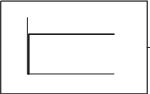
\includegraphics[width=0.2\textwidth]{images/PStrecke}
    \caption{Blockschaltbild von P-Strecke}
    \label{fig:PStrecke}
\end{figure}


% ---------------------------------------------------------------------------- %
\subsubsection*{Strecken mit Totzeit}
% ---------------------------------------------------------------------------- %

\"Andert  sich  die  Stellgr\"osse,  wirkt sich  diese  \"Anderung  bei  einer
Strecke  mit Totzeit  erst  nach  einer gewissen  Zeit  auf die  Regelgr\"osse
aus. Mit $T_t$  wird das  Mass der Totzeit  gekennzeichnet. Im Blockschaltbild
(Abb.  \ref{fig:TotZeit}) wird  die  Totzeit durch  ein  Unterbruch am  Anfang
gekennzeichnet.

Totzeiten     verursachen    schnelle     Schwingungen,     da    sich     die
Stellgr\"osse\"nanderung zeitverz\"ogert  auf die  Regelgr\"osse auswirkt. Die
Schwingungen  entstehen  wenn sich  die  Stellgr\"osse  und die  Regelgr\"osse
periodisch \"andern.

\begin{figure}[h!, width=\pagewidth]
    \centering
    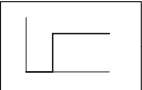
\includegraphics[width=0.2\textwidth]{images/TotZeit}
    \caption{Blockschaltbild von Strecke mit Totzeit}
    \label{fig:TotZeit}
\end{figure}


% ---------------------------------------------------------------------------- %
\subsubsection*{I-Regelstrecke}
% ---------------------------------------------------------------------------- %

Die  I-Regelstrecke  antwortet  auf eine  Stellgr\"ossen\"anderung  mit  einer
fortw\"ahrenden \"Anderung in steigende oder fallende Richtung. Die Begrenzung
dieses   Vorganges  ist   mit  den   systembedingten  Schranken   gegeben. Die
Integrierzeit  $T_i$  ist  ein  Mass  f\"ur  die  Anstiegsgeschwindigkeit  der
Regelgr\"osse  und das  Blockschaltbild  (Abb.  \ref{fig:IStrecke}) zeigt  das
Verhalten sinnbildlich.

\begin{figure}[h!, width=\pagewidth]
    \centering
    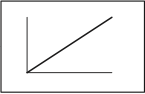
\includegraphics[width=0.2\textwidth]{images/IStrecke}
    \caption{Blockschaltbild von I-Strecke}
    \label{fig:IStrecke}
\end{figure}


% ---------------------------------------------------------------------------- %
\subsection{Regler}
% ---------------------------------------------------------------------------- %

Die Aufgabe  eines Reglers  besteht darin  die zu  regelnde Strecke  mit einem
Stellsignal  so  zu  beeinflussen,  dass der  Wert  der  Regelgr\"osse  gleich
dem  Wert  der F\"uhrungsgr\"osse  entspricht. Der  Regler  besteht aus  einem
Vergleichsglied,  welches  die  Reglerdifferenz  aus  der  Differenz  zwischen
F\"uhrungs-  und Reglergr\"osse  bildet und  dem Reglerglied. Das  Reglerglied
erzeugt aus der Reglerdifferenz die Stellgr\"osse.

Es wird zwischen P-, I- und D-Regler unterschieden.

In diesem Projekt werden die PI- und PID-Regler, welche Kombinationen der oben
genannten Regler sind, behandelt.


% ---------------------------------------------------------------------------- %
\subsubsection{PI-Regler}
% ---------------------------------------------------------------------------- %
Der  PI-Regler   besteht  aus  einer   Parallelschaltung  von  einem   P-  und
einem  I-Regler (Abb.\ref{fig:PIRegler}). Durch  diese Kombination  werden die
Nachteile  beider  Regler  aufgehoben   und  die  Vorteile  (schnell,  stabil)
hervorgehoben. Sein  Verhalten   wird  bildlich  in  dem   Blockschaltbild  in
Abbildung \ref{fig:PIRegler2} dargestellt.

\begin{figure}[h!, width=\pagewidth]
    \centering
    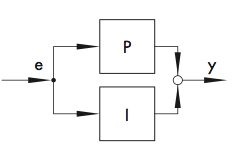
\includegraphics[width=0.4\textwidth]{images/PIRegler1}
    \caption{Parallelschlatung von P-Regler und I-Regler}
    \label{fig:PIRegler1}
\end{figure}

\begin{figure}[h!, width=\pagewidth]
    \centering
    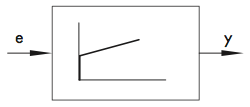
\includegraphics[width=0.4\textwidth]{images/PIRegler2}
    \caption{Blockschaltbild von PI-Regler}
    \label{fig:PIRegler2}
\end{figure}


% ---------------------------------------------------------------------------- %
\subsubsection{PID-Regler}
% ---------------------------------------------------------------------------- %

Wird    dem    PI-Regler    ein    D-Anteil    parallel    geschaltet    (Abb.
\ref{fig:PRDRegler1}), entsteht  der PID-Regler. Der  PID-Regler ist  ein sehr
oft verwendeter  Regler, da durch  den D-Anteil die Regelgr\"osse  rascher den
Sollwert erreicht  und der Einschwingvorgang schneller  abgeschlossen ist. Das
Blockschaltbild  zeigt dieses  Verhalten (Abb.\ref{fig:PID})  anschaulich. Der
PID-Regler  ist   geeignet  f\"ur  Regelstrecken  h\"oherer   Ordnung,  welche
m\"oglichst  schnell  und  ohne bleibende  Regelabweichungen  geregelt  werden
m\"ussen.

\begin{figure}[h!, width=\pagewidth]
    \centering
    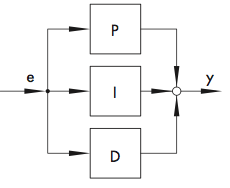
\includegraphics[width=0.4\textwidth]{images/PRDRegler1}
    \caption{Parallelschaltung von P-, I-, und D-Regler}
    \label{fig:PRDRegler1}
\end{figure}

\begin{figure}[h!, width=\pagewidth]
    \centering
    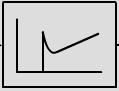
\includegraphics[width=0.4\textwidth]{images/PID}
    \caption{Blockschaltbild des PID-Reglers}
    \label{fig:PID}
\end{figure}
